\documentclass[11pt]{article}
\usepackage[utf8]{inputenc}
\usepackage[T1]{fontenc}
\usepackage[margin=1in]{geometry}
\usepackage{amsmath,amssymb,amsthm}
\usepackage{booktabs}
\usepackage{array}
\usepackage{url}
\usepackage{microtype}
\usepackage{graphicx}
\usepackage{caption}
\usepackage[hidelinks]{hyperref}
\makeatletter\g@addto@macro{\UrlBreaks}{\do\_\do\.}\makeatother
\DeclareUrlCommand\lean{\urlstyle{tt}}
\emergencystretch=3em
\newcommand{\ETriTwo}{0.3935333668}
\newcommand{\ESqTwo}{0.4009647699}
\newcommand{\DSqTwo}{7.43\times10^{-3}}
\newcommand{\TruncTwo}{1.4\times10^{-8}}
\newcommand{\BoxVsSumTwo}{2.1\times10^{-14}}
\newcommand{\ETriOne}{1.6076092172}
\newcommand{\ESqOne}{1.6171455730}
\newcommand{\DSqOne}{9.54\times10^{-3}}
\newcommand{\TruncOne}{4.2\times10^{-5}}
\newcommand{\BoxVsSumOne}{7.8\times10^{-14}}
\newcommand{\PosGap}{5.2\times10^{-14}}
\newcommand{\NoisyGap}{2.5\times10^{-14}}
\newcommand{\HessMin}{0.0236}
\newcommand{\SqNeg}{72}
\newcommand{\SqAfterGap}{2.22\times10^{-3}}
\newcommand{\POneTwo}{pass}
\newcommand{\PTwoTwo}{pass}
\newcommand{\IncommTwo}{pass}
\newcommand{\UndercutsTwo}{0}
\newcommand{\RelaxTwo}{100}
\newcommand{\PerfTwoHF}{1}
\newcommand{\RunsTwoHF}{20}
\newcommand{\QDefTwoHF}{15}
\newcommand{\MinGapTwoHF}{7.6\times10^{-14}}
\newcommand{\PerfTwoUni}{1}
\newcommand{\RunsTwoUni}{20}
\newcommand{\QDefTwoUni}{14}
\newcommand{\MinGapTwoUni}{8.5\times10^{-14}}
\newcommand{\IncommMinTwo}{9.6\times10^{-4}}
\newcommand{\POneOne}{pass}
\newcommand{\PTwoOne}{FAIL}
\newcommand{\IncommOne}{pass}
\newcommand{\UndercutsOne}{0}
\newcommand{\RelaxOne}{50}
\newcommand{\PerfOneHF}{0}
\newcommand{\RunsOneHF}{10}
\newcommand{\QDefOneHF}{8}
\newcommand{\MinGapOneHF}{5.8\times10^{-5}}
\newcommand{\PerfOneUni}{2}
\newcommand{\RunsOneUni}{10}
\newcommand{\QDefOneUni}{8}
\newcommand{\MinGapOneUni}{1.9\times10^{-14}}
\newcommand{\IncommMinOne}{3.1\times10^{-4}}
\newcommand{\DiskOpenInt}{0.086}
\newcommand{\DiskOpenEdge}{0.965}
\newcommand{\DiskOpenPsi}{0.913}
\newcommand{\DiskOpenR}{10.81}
\newcommand{\DiskClosedInt}{0.033}
\newcommand{\DiskClosedEdge}{0.602}
\newcommand{\DiskClosedPsi}{0.931}
\newcommand{\DiskClosedR}{9.89}
\newcommand{\LedgerClaims}{16}
\newcommand{\LedgerBlocks}{0}
\newcommand{\LedgerFlags}{6}
\newcommand{\LedgerExit}{1}

\newtheorem{theorem}{Theorem}
\newcommand{\R}{\mathbb{R}}

\title{Planar universal optimality, tiered:\\ kernel-checked consequences, a non-uniqueness theorem,\\ and a CVODE $N$-body consistency check for the Yukawa interaction}
\author{Xavier Callens (SocrateAI Lab)}
\date{Preprint v2, 2026-10-11 (v1: doi:10.5281/zenodo.23293112)}
\hypersetup{pdftitle={Planar universal optimality, tiered}, pdfauthor={Xavier Callens}}

\begin{document}
\maketitle
\begin{center}
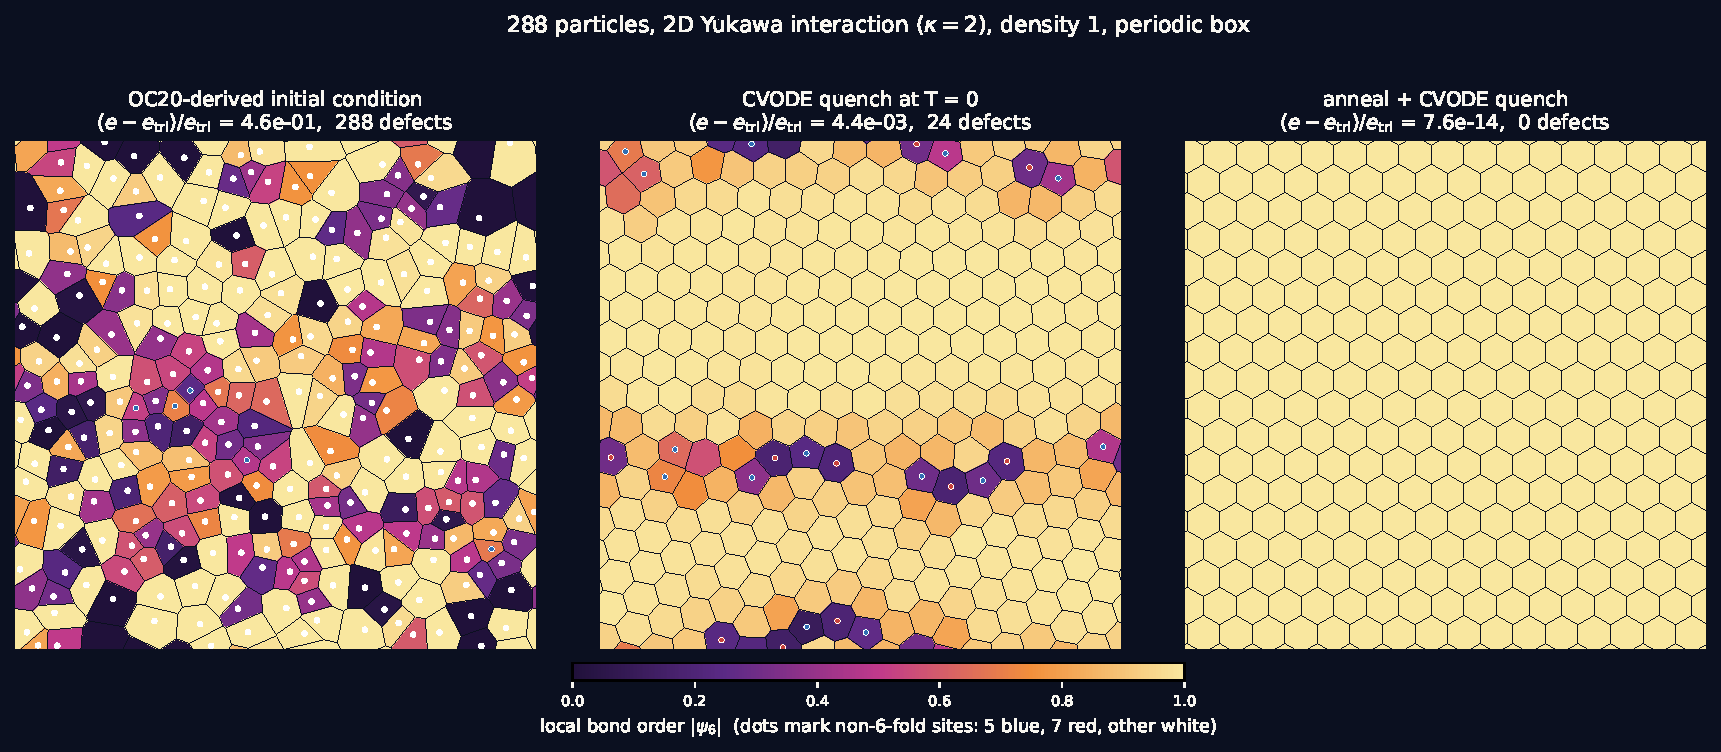
\includegraphics[width=\textwidth]{figures/cover.pdf}
\captionof{figure}{Cover. Three stages of one CVODE study (Tier~X), Voronoi cells coloured by local hexagonal order
$|\psi_6|$, with 5-fold (blue) and 7-fold (red) defects marked. Left: a disordered initial condition derived from the
Hugging Face OC20 dataset. Middle: its zero-temperature CVODE quench, a defected local minimum. Right: an annealed run
followed by a CVODE quench, which reaches the perfect triangular lattice. Every panel is regenerated from a published
seed by \texttt{yukawa\_crystal snapshot}.}\label{fig:cover}
\end{center}

\begin{abstract}
The openai/math release contains a Lean~4 proof that the triangular lattice minimises the lower $g$-energy among all
locally finite planar configurations of density one, for every smooth completely monotone $g$~\cite{oai}. We file every
claim we make about it in a claim ledger with the tiers of the SocrateAI-Scientific-Elenchus method~\cite{elenchus}:
\textbf{A} kernel-checked, \textbf{L} cited literature, \textbf{C} argument, \textbf{X} floating-point
exploration, which may steer but may never support a claim. At Tier~A, conditional only on the fidelity of upstream's
definitions and of our transcription, we prove in Lean that the rescaled triangular lattice is universally optimal at
every density in the sense of Cohn--Kumar--Miller--Radchenko--Viazovska's (CKMRV) Definition~1.3, stated with
upstream's lower energy. That is weaker than their notion, which also requires the energy to exist as a limit. We also
formalise the remark that follows CKMRV's Theorem~1.4, which upstream also notes: universal optima are not unique among
all configurations, because the lattice with one vacancy is another and is not an isometric image of the lattice. In
this formulation only the minimum value is determined, not the minimiser. At Tier~X we run an overdamped $N$-body relaxation
for the 2D Yukawa interaction, which is in the theorem's class (Tier~C), with the CVODE solver of rusty-SUNDIALS, from
initial conditions derived from the Hugging Face OC20 dataset. The preregistered falsifiable prediction, that no
relaxed periodic configuration falls below the triangular-lattice energy, is reported with its controls. It is
consistency evidence, not proof. The Elenchus ledger gate reports \LedgerBlocks{} blocking findings and
\LedgerFlags{} flags (exit \LedgerExit). Each flag marks a Tier~A row whose statement adequacy no human has audited,
so by the method's own publish gate the ledger does not yet pass.
\end{abstract}

\section{Claims and tiers}

Table~\ref{tab:ledger} lists every claim made below, with its tier and its ledger identifier.

\begin{table}[!ht]\centering\small
\begin{tabular}{>{\raggedright\arraybackslash}p{2.1cm}p{0.7cm}p{11.7cm}}
\toprule
Ledger id & Tier & Claim (abbreviated; full statements in \texttt{ledger.json}) \\
\midrule
UO-A-0001 & A & upstream \lean{universal_energy_minimum} (our compile and footprint; definitions AI-audited only)\\
UO-A-0002--4 & A & Riesz admissibility and optimality; finiteness for $s>2$; every density with attainment~\cite{d12}\\
UO-A-0005 & A & \lean{triangular_universally_optimal}: $\rho^{-1/2}A$ is \lean{UniversallyOptimal} for every $\rho>0$\\
UO-A-0006 & A & \lean{universal_optimum_not_unique}: $A\setminus\{0\}$ is universally optimal and not an isometric image of $A$\\
UO-L-0001--6 & L & CKMRV Definition~1.3, uniqueness remark, history, composition footnote, lattice energy~\cite{ckmrv}; upstream scope remark~\cite{oai}\\
UO-C-0001 & C & the 2D Yukawa interaction is completely monotone in $r^2$\\
UO-C-0002 & C & the interpretation of UO-A-0006 (what it does and does not refute)\\
UO-X-000$n$ & X & CVODE $N$-body study, controls, disk study (\texttt{claim\_licence: false})\\
\bottomrule
\end{tabular}
\caption{The claim ledger. A row may not be cited above its tier, and no row is filed above anything it rests on;
both are checked mechanically, transitively, by the Elenchus gate. Every row points to a content-addressed evidence
blob (compiled axiom output with source hashes, primary-source excerpts with line numbers, argument text, or result
files).}\label{tab:ledger}
\end{table}

\section{Tier A: what the kernel checked}

\paragraph{Upstream (UO-A-0001).} With $A$ the triangular lattice of covolume one, $N_R(C)$ the number of points of $C$
in the closed disk of radius $R$, density $\lim N_R/(\pi R^2)$, and lower energy
$E_g(C)=\liminf_R N_R^{-1}\sum_{x\ne y}g(|x-y|^2)$ in $[0,\infty]$, upstream proves
$\sum_{a\in A\setminus0}g(|a|^2)\le E_g(C)$, with equality for $C=A$, for every smooth completely monotone $g$. We
recompiled it with the pinned toolchain (Lean~4.34.1, Mathlib \texttt{d13f23b7}, openai/math \texttt{adc7f124},
unchanged at \texttt{fd4aeeb2}); its footprint is $\{$\lean{propext}, \lean{Classical.choice}, \lean{Quot.sound}$\}$. The
proof is checked. What is not established by any gate is that these definitions are the intended ones; our item-by-item
comparison with~\cite[Defs.~1.1--1.3]{ckmrv} was done by AI agents and is filed as such.

\paragraph{Earlier corollaries (UO-A-0002--4).} Riesz admissibility, finiteness of the lattice Riesz energy for $s>2$,
and optimality of $\rho^{-1/2}A$ at every density with attainment are in~\cite{d12}.

\paragraph{Universal optimality in the sense of CKMRV (UO-A-0005).} Define, in upstream's notions,
\begin{align*}
\mathrm{UO}(\rho,C)\;:\iff\;& C \text{ locally finite},\quad \mathrm{dens}(C)=\rho,\quad\text{and}\\
& \forall g \text{ admissible},\ \forall C' \text{ locally finite of density } \rho:\ E_g(C)\le E_g(C').
\end{align*}
This transcribes~\cite[Def.~1.3]{ckmrv} with one difference: CKMRV also require the energy of $C$ to exist as a limit,
and $\mathrm{UO}$ uses only the $\liminf$, so it is weaker (we do not claim it is strictly weaker; no witness is
filed). For a lattice whose sum $\sum_{x\ne0}g(|x|^2)$ converges absolutely, CKMRV take the energy to be that sum
(UO-L-0005). Given the unformalised fact that the disk averages then converge to it, Theorem~1 yields CKMRV's notion
for $\rho^{-1/2}A$. That step is Tier~C and is not claimed here.
\begin{theorem}[\lean{triangular_universally_optimal}]
For every $\rho>0$, $\mathrm{UO}(\rho,\rho^{-1/2}A)$.
\end{theorem}

\paragraph{Non-uniqueness (UO-A-0006).}
\begin{theorem}[\lean{vacancy_energy}; \lean{vacancy_not_isometric_image};\\ \lean{universal_optimum_not_unique}]
For every admissible $g$, $E_g(A\setminus\{0\})=\sum_{a\in A\setminus0}g(|a|^2)$. Hence $\mathrm{UO}(1,A\setminus\{0\})$, and
there is no isometry $f$ of the plane with $f(A)=A\setminus\{0\}$.
\end{theorem}
\noindent\emph{Proof idea.} Removing one point removes a sub-sum from each disk energy, and the normalisation changes
by $N_R/(N_R-1)\to1$; the $\liminf$ comparison closes with \lean{ENNReal.liminf_mul_le}, and upstream's theorem gives
the reverse inequality. For the isometry statement, isometries of the plane are affine (Mathlib's
\lean{Isometry.affineIsometryOfStrictConvexSpace}), so $f(2a-b)=2f(a)-f(b)$. Write $p$ for \lean{triangularPoint}
and pick $a,b\in A$ with $f(a)=p(1,0)$ and $f(b)=p(2,0)$. Then $2a-b\in A$ and $f(2a-b)=2p(1,0)-p(2,0)=p(0,0)=0$,
contradicting $0\notin A\setminus\{0\}$ (Figure~\ref{fig:vacancy}).

\begin{figure}[!ht]\centering
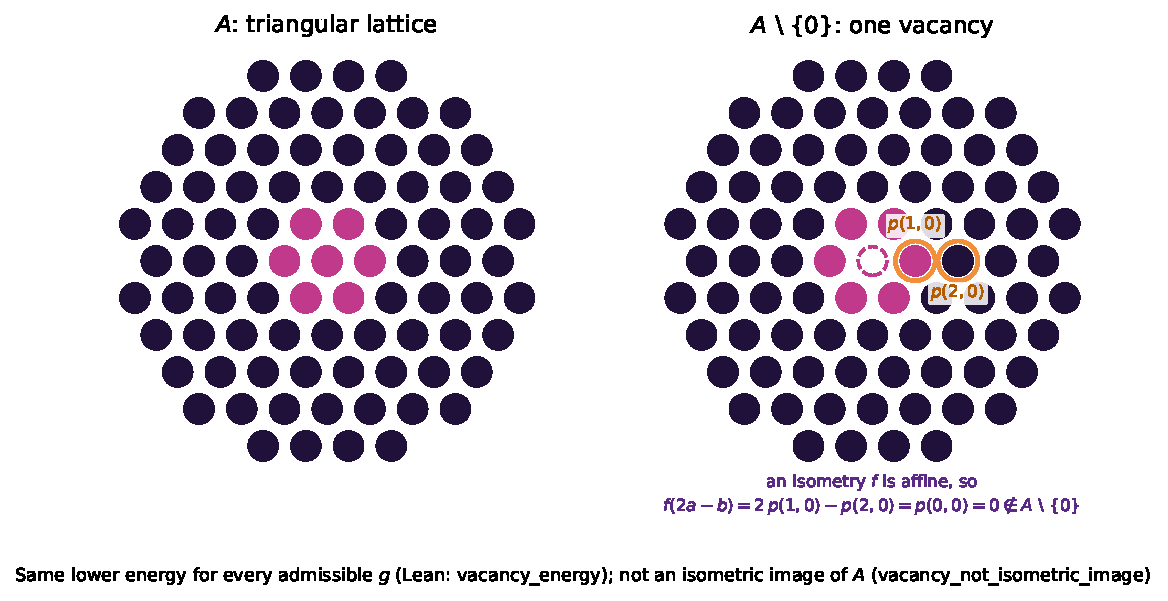
\includegraphics[width=0.86\textwidth]{figures/vacancy.pdf}
\caption{The non-uniqueness theorem (UO-A-0006). Removing the origin leaves the lower energy unchanged for every
admissible $g$. No isometry carries $A$ onto $A\setminus\{0\}$: an isometry of the plane is affine, so it would send
$2a-b$ to $2p(1,0)-p(2,0)=0$.}\label{fig:vacancy}
\end{figure}

This is the remark after~\cite[Thm.~1.4]{ckmrv} (UO-L-0002), also noted by upstream (``it identifies the minimum
value, not all minimizers''~\cite[\S1]{oai}, UO-L-0006), now as a theorem in this setting. Its interpretation (UO-C-0002) is
Tier~C: in the lower-energy formulation over \emph{all} locally finite configurations, ``the minimiser is the
triangular lattice'' is false, and only the minimum value is pinned down. Uniqueness among \emph{periodic}
configurations, which CKMRV prove in dimensions 8 and 24, is not claimed by upstream for dimension~2 and is not
addressed here.

\paragraph{Gates.} A clean sequential rebuild of the whole chain exits~0 (recorded in the AutoevolveAI commit message
\texttt{d50dfc4}; no build log is committed). The audit file prints 24 footprints: the 22 audited declarations are
within the allowlist, and the 2 planted controls (\lean{sorry}, a custom axiom) are flagged by the same audit. Each layer
was re-verified by a separate instance of the same AI model that recompiled it and wrote its own controls. That is
producer$\ne$verifier, not human review.

\section{Tier L: what is known}
Per CKMRV's own text (UO-L-0003): Ventevogel and Nijboer proved universal optimality of $\mathbb Z$ in dimension~1
(Cohn and Kumar gave another proof); before CKMRV no universal optimum was proved in any dimension $>1$; CKMRV proved
it for $E_8$ and the Leech lattice; and universal optimality of the hexagonal lattice ``in full generality is an
important open problem''. So, per CKMRV, dimension~1 was settled before dimensions 8 and 24, and dimension~2 was
then the lowest open case.

\section{Tier C: why the Yukawa interaction is in the class}
$V(r)=e^{-\kappa r}/r$ is $g(t)=e^{-\kappa\sqrt t}/\sqrt t$ with $t=r^2$. Here $t^{-1/2}$ is completely monotone;
$e^{-\kappa\sqrt t}=p\circ q$ with $p(u)=e^{-\kappa u}$ completely monotone and $q'(t)=\tfrac12t^{-1/2}$ completely
monotone, hence completely monotone by~\cite[footnote~2]{ckmrv} (UO-L-0004); and products of completely monotone
functions are completely monotone (Leibniz). So upstream's theorem, if its definitions are faithful, predicts that no
density-one configuration has Yukawa energy below the triangular lattice's. This argument is not kernel-checked
(UO-C-0001), and so the numerics below rest on Tier~C, not on Tier~A.

\section{Tier X: a CVODE $N$-body consistency check}

\paragraph{Instrument.} rusty-SUNDIALS~\cite{rusty}, crate \texttt{qf-yukawa-crystal}. $N=288$ particles in a periodic
rectangle that holds the triangular lattice $16\times18$ exactly at density~1; shifted-force Yukawa with cutoff
$r_c=8$ (minimum image), $\kappa=2$ ($V(r_c)=\TruncTwo$) and $\kappa=1$ ($V(r_c)=\TruncOne$). The truncated
potential is not exactly completely monotone beyond $r_c$; that is a disclosed approximation. Overdamped relaxation
$\dot x=-\nabla E$ is integrated by CVODE (BDF) with the analytic Jacobian $-\nabla^2E$ until $\max|F|<10^{-9}$, and
minima are checked by the Hessian spectrum (cyclic Jacobi). Two packages named in common descriptions of this pipeline
were not used: rusty-SUNDIALS has no KINSOL port, and its IDA crate documents itself as a fixed-step prototype.
Annealing is overdamped Langevin (Euler--Maruyama) outside SUNDIALS, because a stochastic equation is not an ODE,
followed by a CVODE quench.

\paragraph{Initial conditions.} Twenty disordered configurations derived from the Hugging Face dataset
\texttt{colabfit/OC20\_IS2RES\_val\_id}~\cite{oc20} (CC-BY-4.0): random OC20 structures, rotated uniformly in 3D,
projected, rescaled and accepted with a minimum separation. Twenty uniform random configurations serve as a second
family. We do not claim that either is more realistic; the dataset supplies disorder, not physics. Machine-learned
interatomic potentials were deliberately not used: they model atomic chemistry, not a completely monotone pair
potential, and cannot test this theorem.

\paragraph{Preregistration.} The predictions and controls were committed (\texttt{636c514}) before the solver code
(\texttt{968b0f2}) and before the results (\texttt{1f46e70}) were committed. Git cannot show that no local run
preceded the preregistration commit. P1: no
relaxed configuration has energy per particle below $e_{\rm tri}$ by more than $10^{-9}$ relative. P2: at least one
annealed run per family reaches the perfect lattice. P3: $T=0$ quenches mostly end in defected local minima, which is
a property of gradient flow and not evidence against the theorem. \emph{Deviations from the preregistration.} (a) The
coordination cutoff is $1.35\,d_0$, with $d_0$ the median nearest-neighbour distance of the configuration, not the
registered $1.4a$. (b) At $\kappa=1$ ten initial conditions per family were run, and five incommensurate controls,
instead of the registered twenty per family; the number of incommensurate runs was not registered. (c) The incommensurate control's automatic pass test checks only that every state
is above $e_{\rm tri}$; that the states are defected, also registered, is read from the table (all are).

\begin{figure}[!ht]\centering
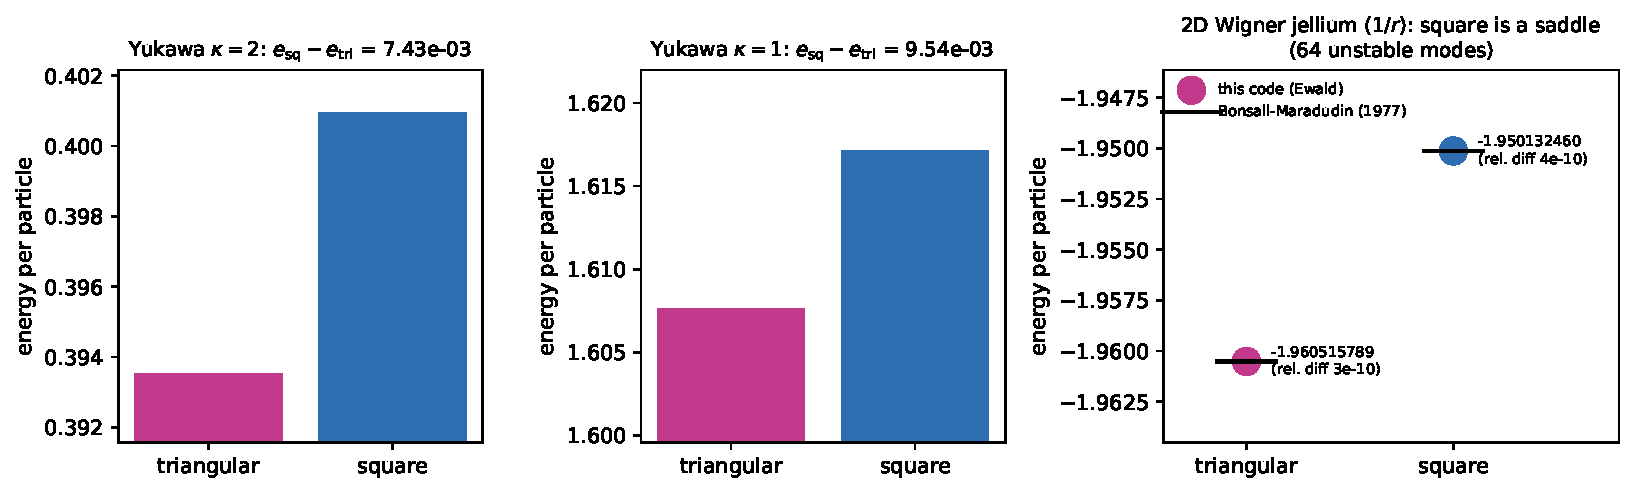
\includegraphics[width=\textwidth]{figures/lattices.pdf}
\caption{Reference energies per particle at density~1. Left and middle: Yukawa, triangular below square at both
$\kappa$. Right: the jellium extension (Section~\ref{sec:extension}), where this code's Ewald energies match Bonsall
and Maradudin~\cite{bm} to $\le 4\times10^{-10}$ and the square lattice is a saddle point.}\label{fig:lattices}
\end{figure}

\paragraph{Controls.} References: $e_{\rm tri}=\ETriTwo$ and $e_{\rm sq}=\ESqTwo$ at $\kappa=2$
($e_{\rm sq}-e_{\rm tri}=\DSqTwo$); the periodic box reproduces the direct lattice sum to $\BoxVsSumTwo$. A perfect
lattice stays put (relative gap $\PosGap$); a lattice with $0.1a$ noise relaxes back (gap $\NoisyGap$); the Hessian at
the lattice has exactly two zero translation modes and smallest other eigenvalue $\HessMin$. Negative controls: the
square lattice is a stationary point with $\SqNeg$ negative Hessian eigenvalues (a saddle) and relaxes below its energy;
in a box that cannot hold the triangular lattice the relaxed states keep defects and stay above $e_{\rm tri}$
(\IncommTwo).

\paragraph{Results.} Table~\ref{tab:num}. \textbf{P1} (the falsifiable prediction): \POneTwo{} at $\kappa=2$, with
\UndercutsTwo{} undercuts in \RelaxTwo{} relaxations (\RelaxCtlTwo{} of them in the incommensurate control box), and
\POneOne{} at $\kappa=1$, with \UndercutsOne{} undercuts in \RelaxOne{} (\RelaxCtlOne{} control). The lowest annealed gaps, $\MinGapTwoHF$ (OC20-derived) and $\MinGapTwoUni$ (uniform) at $\kappa=2$, are the
lattice itself to round-off. \textbf{P2}: \PTwoTwo{} at $\kappa=2$, but narrowly: \PerfTwoHF{} of \RunsTwoHF{}
(OC20-derived) and \PerfTwoUni{} of \RunsTwoUni{} (uniform) annealed runs reached the perfect lattice. At $\kappa=1$
P2 \emph{fails as preregistered}: \PerfOneHF{} of \RunsOneHF{} and \PerfOneUni{} of \RunsOneUni{}. The other annealed
runs end in defected local minima or in defect-free states above $e_{\rm tri}$. The annealing schedule is a weak
instrument, and this failure says nothing about the theorem in either direction. \textbf{P3}, as expected: \QDefTwoHF{}
of \RunsTwoHF{} and \QDefTwoUni{} of \RunsTwoUni{} $T=0$ quenches at $\kappa=2$ keep defects. The remainder are
defect-free but above $e_{\rm tri}$; their structure was not analysed. Every run converged to $\max|F|<10^{-9}$. The
final Hessian was computed for the \HessCheckedTwo{} ($\kappa=2$) and \HessCheckedOne{} ($\kappa=1$) non-control runs.
\HessNegTwo{} and \HessNegOne{} of them have an eigenvalue below $-10^{-9}\lambda_{\max}$. All have exactly two
translation modes ($|\lambda|\le\HessTransTwo$ at $\kappa=2$, $\le\HessTransOne$ at $\kappa=1$), and every
other eigenvalue is at least $\HessThirdTwo$ ($\kappa=2$) and $\HessThirdOne$ ($\kappa=1$). These end states are
therefore strict local minima modulo translation. The incommensurate-box and disk runs were not Hessian-checked. The
negative control behaves as it must: in the incommensurate box every relaxed state is defected and at least
$\IncommMinTwo$ above $e_{\rm tri}$. At $\kappa=2$ the two initial-condition families behave alike. At $\kappa=1$
they differ (Table~\ref{tab:num}), with small counts. Nothing in these runs depends on the dataset's chemistry: it
supplied disorder only.

\begin{table}[h]\centering\scriptsize\setlength{\tabcolsep}{3pt}
\begin{tabular}{llrrrrrrr}
\toprule
& family / stage & runs & perfect & defected & min rel.\ gap & max rel.\ gap & not conv. & Hess.$<0$\\
\midrule
$\kappa=2$ & incomm.\ box (ctl), anneal + quench & 10 & 0 & 10 & $9.60\times10^{-4}$ & $1.73\times10^{-3}$ & 0 & 0 \\
$\kappa=2$ & incomm.\ box (ctl), $T=0$ quench & 10 & 0 & 10 & $9.60\times10^{-4}$ & $5.67\times10^{-3}$ & 0 & 0 \\
$\kappa=2$ & OC20-derived, anneal + quench & 20 & 1 & 11 & $7.60\times10^{-14}$ & $2.53\times10^{-3}$ & 0 & 0 \\
$\kappa=2$ & OC20-derived, $T=0$ quench & 20 & 0 & 15 & $1.84\times10^{-4}$ & $4.89\times10^{-3}$ & 0 & 0 \\
$\kappa=2$ & uniform, anneal + quench & 20 & 1 & 11 & $8.48\times10^{-14}$ & $2.39\times10^{-3}$ & 0 & 0 \\
$\kappa=2$ & uniform, $T=0$ quench & 20 & 0 & 14 & $1.84\times10^{-4}$ & $6.04\times10^{-3}$ & 0 & 0 \\
$\kappa=1$ & incomm.\ box (ctl), anneal + quench & 5 & 0 & 5 & $3.09\times10^{-4}$ & $6.25\times10^{-4}$ & 0 & 0 \\
$\kappa=1$ & incomm.\ box (ctl), $T=0$ quench & 5 & 0 & 5 & $3.10\times10^{-4}$ & $1.07\times10^{-3}$ & 0 & 0 \\
$\kappa=1$ & OC20-derived, anneal + quench & 10 & 0 & 5 & $5.77\times10^{-5}$ & $1.22\times10^{-3}$ & 0 & 0 \\
$\kappa=1$ & OC20-derived, $T=0$ quench & 10 & 0 & 8 & $5.77\times10^{-5}$ & $1.70\times10^{-3}$ & 0 & 0 \\
$\kappa=1$ & uniform, anneal + quench & 10 & 2 & 3 & $1.93\times10^{-14}$ & $8.51\times10^{-4}$ & 0 & 0 \\
$\kappa=1$ & uniform, $T=0$ quench & 10 & 1 & 8 & $3.96\times10^{-14}$ & $1.22\times10^{-3}$ & 0 & 0 \\
\bottomrule

\end{tabular}
\caption{CVODE relaxations. ``perfect'': zero defects and $|e-e_{\rm tri}|<10^{-8}|e_{\rm tri}|$. Relative gap
$(e-e_{\rm tri})/e_{\rm tri}$. ``Hess.$<0$'': runs whose final Hessian has an eigenvalue below $-10^{-9}\lambda_{\max}$, over runs whose Hessian
was computed (n/a: not
computed). The incommensurate
family uses a square box and is a negative control. Tier~X throughout.}\label{tab:num}
\end{table}

\begin{figure}[!ht]\centering
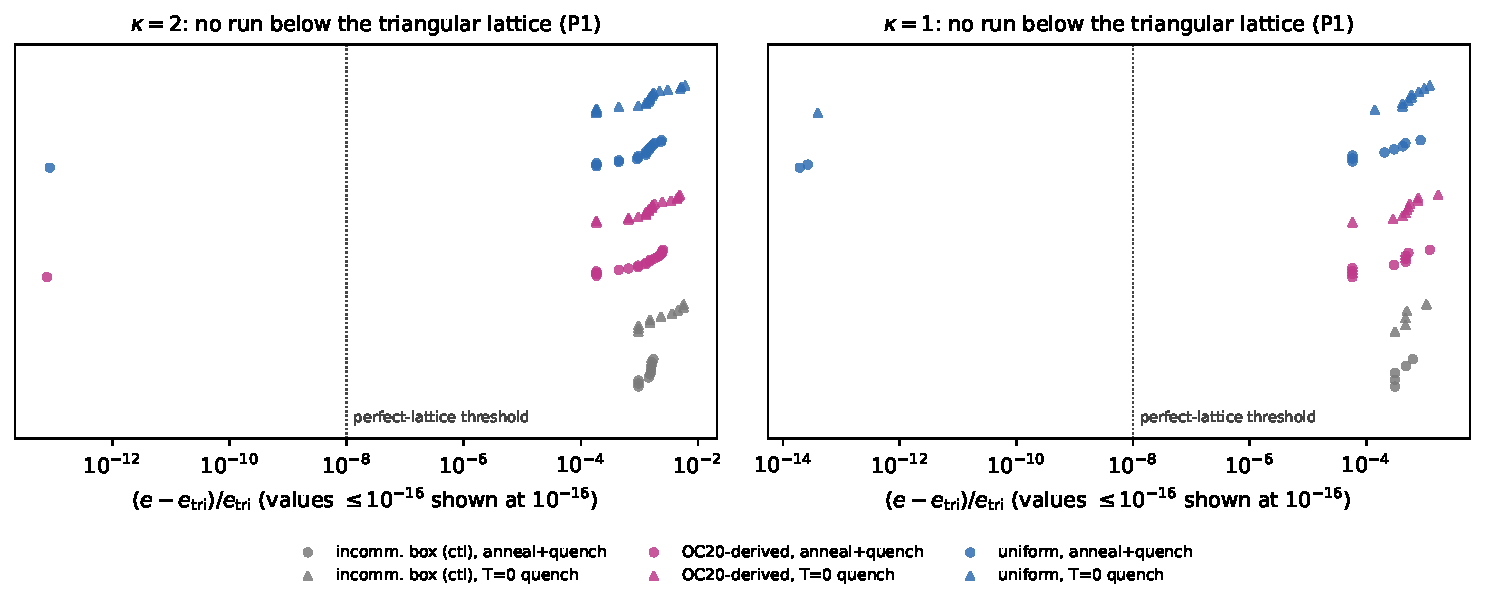
\includegraphics[width=\textwidth]{figures/gaps.pdf}
\caption{Every relaxation's relative energy gap to the triangular lattice, one marker per run, on a logarithmic axis.
P1 concerns the sign of the gap, which the summary script checks for every run (no gap is negative). Markers at the
far left are runs that reached the lattice to round-off. Generated from \texttt{main\_kappa\{2,1\}.jsonl}.}\label{fig:gaps}
\end{figure}

\paragraph{Open versus closed disk.} $N=300$, $\kappa=2$, annealed and quenched: harmonic bowl (open) versus soft
wall (closed). Interior defect fraction \DiskOpenInt{} (open) versus \DiskClosedInt{} (closed); edge \DiskOpenEdge{}
versus \DiskClosedEdge; interior mean $|\psi_6|$ \DiskOpenPsi{} versus \DiskClosedPsi. The comparison is confounded:
the bowl produces a non-uniform density, the closed disk compresses particles against the wall, and the two ``edge''
layers (within two spacings of the outermost particle) contain different numbers of particles. It describes
finite-size edge effects in these two set-ups and is not a controlled measurement of either. It is not a test of whether upstream's closed-disk counting differs from an open-disk one, which is a question
about measure-zero boundary terms in a limit. Figure~\ref{fig:disks} shows one run of each.

\begin{figure}[!ht]\centering
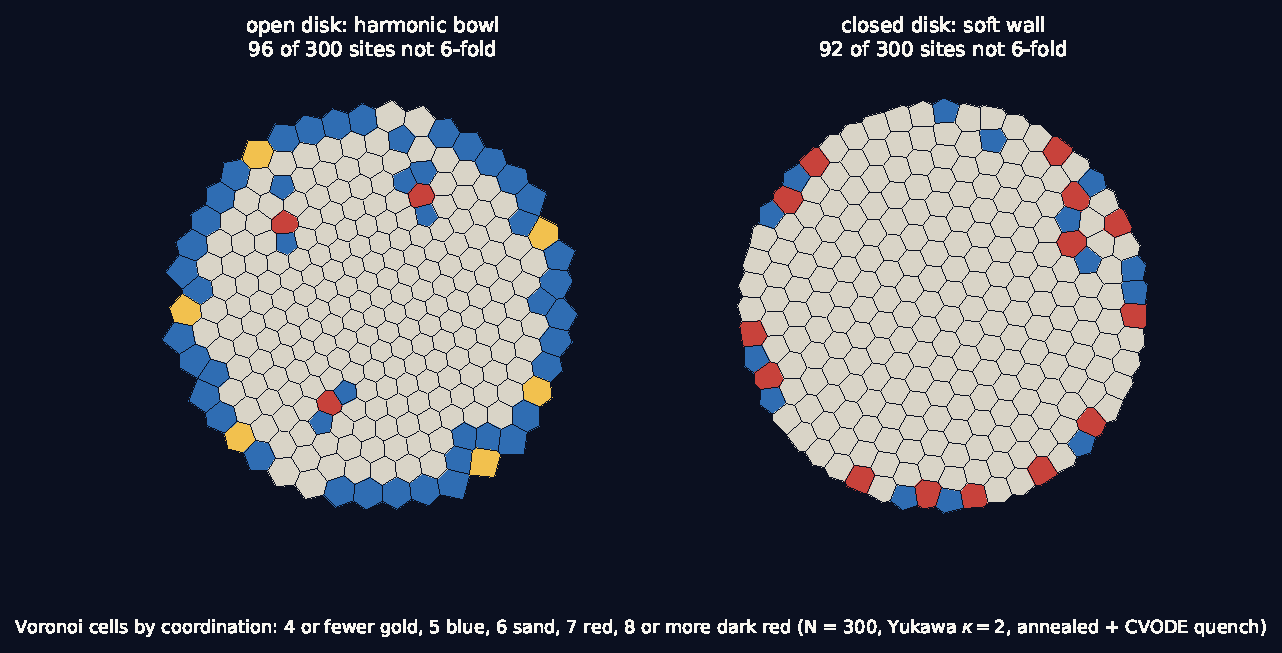
\includegraphics[width=0.92\textwidth]{figures/disks.pdf}
\caption{Open (harmonic bowl) versus closed (soft wall) disk, $N=300$: Voronoi cells coloured by coordination.
Defects concentrate at the edge in both cases, with a near-triangular interior. One run each (\texttt{disk\_00},
regenerated from its published seed); the averages are in the text. Tier~X, and confounded as stated.}\label{fig:disks}
\end{figure}

\section{Extension: long-range interactions and jellium (Tier~X, in progress)}\label{sec:extension}
For $0<s\le2$ and for the logarithm, the raw lattice sum diverges. The comparison of Section~2 then reads $E(C)=\infty$
for every competitor and says nothing. Upstream's manuscript treats this range through renormalized energies against a
neutralizing background (its Section~8, after Petrache and Serfaty~\cite{ps}): for $0\le s<2$ the triangular lattice
minimizes the renormalized energy, and the jellium minimum equals it up to normalisation~\cite{oai}. That corollary is
\emph{not} in upstream's Lean. As a first, numerical step we treat $s=1$, the classical 2D electron gas (Wigner
crystal), by Ewald summation in the same periodic box, with CVODE relaxation and a preregistration (rusty-SUNDIALS
\texttt{e706f85}) committed before the code. Its controls pass: the triangular and square Madelung energies equal
Bonsall and Maradudin's~\cite{bm} to $\le4\times10^{-10}$ relative (Figure~\ref{fig:lattices}); the energy does not
change over a $4\times$ range of the Ewald parameter; and the square lattice is a saddle point with 64 unstable modes,
consistent with the imaginary phonon branch reported in~\cite{bm}. The relaxation study (prediction J1: no relaxed
configuration below the triangular Madelung energy) is reported in the companion record when it completes. The $s=2$
endpoint is outside upstream's statement. The formal targets for this range (a heat-trace comparison, and the
Laplace-transform step of upstream's Lemma ``Heat comparison across period lattices'') are listed with priors in
\texttt{docs/EXTENSION\_RENORMALIZED\_JELLIUM\_2026-10-11.md}.

\section{Laboratory protocols (Tier~C proposals)}\label{sec:lab}
The theorem is about exact potentials and infinite configurations. A laboratory has finite temperature, finite $N$,
polydispersity and imperfect interaction laws. Experiments therefore cannot test the Lean statement. What they can do
is test whether real two-dimensional repulsive systems behave as the theorem and our numerics suggest. Each protocol
below is a proposal (Tier~C); none has been run. All four share one analysis script,
\texttt{lab/lab\_analysis.py}, which takes tracked particle coordinates and computes the same observables as the
simulations. Density comes from the mean Voronoi cell area, coordination from the $1.35\,d_0$ rule; the script also
gives the local and global $|\psi_6|$ and the interaction energy per interior particle for a stated law, compared with
the triangular lattice at the same density. Its self-test passes: a perfect lattice gives gap $6\times10^{-14}$ in any
length unit, thermal noise raises the energy above the lattice, and a square lattice is detected and placed above it.
Every protocol should be preregistered with that script, a predicted bracket, and the kill criterion below.

\paragraph{L1. Superparamagnetic colloids at a flat air--water interface (Riesz $s=3$).} Following Zahn, Wille,
Maret, Sengupta and Nielaba~\cite{zahn}, a perpendicular field $B$ induces parallel dipoles. The pair energy is
$\propto\chi^2B^2/r^3$, a Riesz potential with $s=3$: in the theorem's class, with finite lattice energy (D1b). This
is the most direct realisation of D1.
\emph{Procedure.} Ramp $B$ slowly from the fluid to the crystal (the laboratory analogue of annealing) at fixed area
fraction. Track positions by video microscopy, and record $\chi$ and $B$ so that the law's prefactor is known.
\emph{Predictions.}
\begin{itemize}
\item (a) At large coupling, $|\psi_6|\to1$ and the defect fraction $\to0$ in the interior.
\item (b) The measured dipolar energy per interior particle exceeds the triangular value at the measured density, by
an amount that shrinks as $B$ grows (the thermal excess).
\item (c) A particle removed with optical tweezers leaves a vacancy that relaxes locally, without global
restructuring.
\item (d) A square arrangement imposed with holographic tweezers and then released relaxes away from square. This is
the laboratory version of our square-saddle control.
\end{itemize}
\emph{Kill criterion.} A slowly ramped, defect-free interior whose dipolar energy lies below the triangular value
beyond the measurement error, with the law's prefactor independently confirmed.

\paragraph{L2. Dusty-plasma monolayer (Yukawa).} Thomas et al.~\cite{thomas} observed Coulomb crystallization of
charged microparticles levitated in a plasma sheath. The interaction is screened Coulomb (Yukawa), and the radial
confinement is close to parabolic, the analogue of our open bowl.
\emph{Procedure.} Measure $\kappa$ and the coupling from the phonon spectrum or the pair correlation. Image the
monolayer, run the shared script, and simulate our bowl model at the measured $\kappa$ and $N$.
\emph{Predictions.} A near-triangular interior, with defects concentrated at the rim. The interior defect fraction is
compared with the simulation at matched $\kappa$ and $N$ (Figure~\ref{fig:disks}, left).
\emph{Confounds.} Ion-wake attraction (non-reciprocal forces), neutral drag and vertical oscillations. Any of these
moves the system outside the theorem's class.

\paragraph{L3. Charged colloids in circular, hexagonal and square cavities (closed disk).} Bubeck, Neser, Bechinger
and Leiderer~\cite{bubeck} confined 10--100 screened-Coulomb colloids in lithographic cavities and found structures
dominated by the cavity shape.
\emph{Procedure.} Repeat the circular-cavity case at $N\approx300$ and image the interior; compare with our
closed-wall runs at matched $N$ and wall stiffness.
\emph{Prediction.} The edge defect fraction exceeds the interior one, as in Figure~\ref{fig:disks}, right. Compared
with L2 at matched $N$ and density, this is the experimental open-versus-closed comparison.

\paragraph{L4. Electrons on liquid helium (jellium, $s=1$).} Grimes and Adams~\cite{grimes} observed the
liquid-to-crystal transition of a classical 2D sheet of electrons held above liquid helium. The electrodes supply the
neutralizing background, so this is the jellium case of Section~\ref{sec:extension}.
\emph{Prediction.} The crystal is triangular. The evidence in~\cite{grimes} is spectroscopic, not a direct image, so a
test here compares spectroscopic signatures with the triangular Madelung and phonon structure~\cite{bm}. Direct
imaging of the lattice would need a different detection method, which we do not specify.

\section{Limitations}
\begin{enumerate}
\item No human has audited whether upstream's definitions, or ours, express the intended mathematics; the ledger flags
every Tier~A row for this.
\item $\mathrm{UO}$ is weaker than CKMRV's universal optimality (it does not require the energy limit to exist).
\item Uniqueness among periodic configurations in dimension~2 is not claimed by upstream and was not attempted.
\item The Yukawa step is Tier~C; the numerics are Tier~X and support no claim.
\item Finite $N$, truncated potential, heuristic annealing: P2 can fail for reasons that have nothing to do with the
theorem.
\end{enumerate}

\paragraph{Reproducibility.} Lean: AutoevolveAI \texttt{formal\_cert/Triangular/}; LeanMaster release
\texttt{v3.48.1}. Numerics: rusty-SUNDIALS results commit \texttt{1f46e70}; summary regenerated by \texttt{scripts/summarize.py} at
\texttt{e1a6083}. Ledger and evidence:
\texttt{results/discovery/ledger/} (gate: \texttt{tools/ledger.py} of~\cite{elenchus}, exit \LedgerExit{}:
\LedgerClaims{} claims, \LedgerBlocks{} blocks, \LedgerFlags{} flags).

\paragraph{Version history.} v1 (doi:10.5281/zenodo.23293112): the text, tables and ledger. v2 adds the figures,
all generated by \texttt{make\_figures.py} from the result files and from snapshots that re-run published seeds. It
also adds the jellium extension's preregistration and controls (Section~\ref{sec:extension}) and the laboratory
protocols (Section~\ref{sec:lab}). No v1 result changed.

\paragraph{Publication decision.} The Elenchus publish gate requires the ledger gate to exit~0, and it exits~1
because of the \LedgerFlags{} unaudited-statement flags. The author reviewed the draft and decided to publish with
those flags open, as a preprint, and to seek the statement-adequacy review from the community. Until that review
exists, every Tier~A row should be read as ``the kernel checked the proof; no person has certified that the statement
means what its gloss says''.

\paragraph{AI use.} The proofs, numerics, ledger and text were produced by AI agents (Claude) under the author's
direction; verification runs and the manuscript audit were separate instances of the same model. A DeepSeek-Prover-V2
model (on Cloud Run) was also queried during the Lean work; none of its output was used. The author is responsible
for the content.

\begin{thebibliography}{9}
\bibitem{oai} OpenAI, Universal optimality of the triangular lattice, OpenAI Math Release preprint, 2026-09-23,
\url{https://github.com/openai/math}.
\bibitem{ckmrv} H.~Cohn, A.~Kumar, S.~D.~Miller, D.~Radchenko, M.~Viazovska, Universal optimality of the $E_8$ and
Leech lattices and interpolation formulas, Ann.\ of Math.\ 196 (2022) 983--1082, doi:10.4007/annals.2022.196.3.3.
\bibitem{d12} X.~Callens, Riesz-energy, finiteness and every-density corollaries of the openai/math planar
universal-optimality theorem, kernel-checked in Lean 4, Zenodo (2026), doi:10.5281/zenodo.23285631.
\bibitem{elenchus} X.~Callens, SocrateAI-Scientific-Elenchus,
\url{https://github.com/xaviercallens/SocrateAI-Scientific-Elenchus} (commit \texttt{c9ae8cd}).
\bibitem{rusty} X.~Callens, rusty-SUNDIALS, \url{https://github.com/xaviercallens/rusty-SUNDIALS}.
\bibitem{bm} L.~Bonsall, A.~A.~Maradudin, Some static and dynamical properties of a two-dimensional Wigner crystal,
Phys.\ Rev.\ B 15 (1977) 1959, doi:10.1103/PhysRevB.15.1959; Madelung values as recalculated in arXiv:2103.01622.
\bibitem{ps} M.~Petrache, S.~Serfaty, Crystallization for Coulomb and Riesz interactions as a consequence of the
Cohn--Kumar conjecture, Proc.\ AMS 148 (2020) 3047--3057, doi:10.1090/proc/15003.
\bibitem{zahn} K.~Zahn, A.~Wille, G.~Maret, S.~Sengupta, P.~Nielaba, Elastic properties of 2D colloidal crystals
from video microscopy, Phys.\ Rev.\ Lett.\ 90 (2003) 155506, doi:10.1103/PhysRevLett.90.155506.
\bibitem{thomas} H.~Thomas, G.~E.~Morfill, V.~Demmel, J.~Goree, B.~Feuerbacher, D.~M\"ohlmann, Plasma crystal:
Coulomb crystallization in a dusty plasma, Phys.\ Rev.\ Lett.\ 73 (1994) 652, doi:10.1103/PhysRevLett.73.652.
\bibitem{bubeck} R.~Bubeck, S.~Neser, C.~Bechinger, P.~Leiderer, Structure and dynamics of two-dimensional colloidal
crystals in confined geometry, Prog.\ Colloid Polym.\ Sci.\ (1998) 41--45, doi:10.1007/BFb0118046.
\bibitem{grimes} C.~C.~Grimes, G.~Adams, Evidence for a liquid-to-crystal phase transition in a classical,
two-dimensional sheet of electrons, Phys.\ Rev.\ Lett.\ 42 (1979) 795, doi:10.1103/PhysRevLett.42.795.
\bibitem{oc20} L.~Chanussot et al., OC20 IS2RES val id, ColabFit (2024), doi:10.60732/b4005525; Open Catalyst 2020,
ACS Catal.\ 11 (2021) 6059, doi:10.1021/acscatal.0c04525.
\end{thebibliography}
\end{document}
